\chapter{LArIAT: Liquid Argon In A Testbeam}\label{sec:experimentDescription}

LArIAT, a small Liquid Argon Time Projection Chamber (LArTPC) in a test beam,  is designed to perform an extensive physics campaign centered on charged particle cross section measurements while characterizing the detector performance for future LArTPCs. LArTPC represents one of the most advanced experimental technologies for physics at the Intensity Frontier due to its full 3D-imaging, excellent particle identification and precise calorimetric energy reconstruction. This complex technology however needs a thorough calibration and dedicated measurements of some key quantities to achieve the precision required for the next generation of discoveries at the Intensity Frontier which LArIAT can provide. 

The LArIAT LArTPC is deployed in a dedicated calibration test beamline at Fermilab.
We use the LArIAT beamline to characterize the charge particles before they enter the TPC: the particle type and initial momentum is known from beamline information. The precise calorimetric energy reconstruction of the LArTPC technology enables the measurement of the total differential cross section for  tagged hadrons. 
The Pion-Nucleus and Kaon-Nucleus total hadronic interaction cross section have never been measured before in argon and they are a fundamental step to shed light on light meson interaction in nuclei. Additionally, these measures provides a key input to neutrino physics and proton decay studies in future LArTPC experiments like SBN and DUNE.


%\section{LArIAT \& the Intensity Frontier}
\section{The Particles Path to LArIAT}

LArIAT's home at Fermilab is the Fermilab Test Beam Facility (FTBF), where the experiment characterizes a beam of charge particles downstream from the Meson Center beam line. 

LArIAT's particles history begins in the Fermilab accelerator complex with a beam of protons. The process of protons acceleration develops in gradual stages, see picture \ref{fig:Accelerator}: gaseous hydrogen is ionized in order to form H$^{-}$ ions; these ions are boosted to 750 keV by a Cockroft-Walton accelerator and injected to the Linac linear accelerator that increases their energy up to 400 MeV; then, H$^{-}$ ions pass through a carbon foil and lose the two electrons; the resulting protons are then injected into a rapid cycling synchrotron, called Booster; at this stage protons reach 8 GeV of energy and are compacted into bunches; the next stage of acceleration is the Main Injector, a synchrotron which accelerates the bunches up to 120 GeV; in the Main Injector, several bunches are merged into one and used for the injection in the last stage.


The Fermilab accelerator complex works in supercycles of roughly 60 seconds in duration. The beam is then split by electrostatic septa and delivered at different experimental halls all over the lab. A 120~GeV$/c$ primary proton beam with variable intensity is extracted in four-second ``spills" and sent to the Meson Center beam line. Here, this primary beam is focused onto a tungsten target to create LArIAT's secondary beam. The composition of the secondary particle beam is mainly positive pions. For the LArIAT data considered in this work the secondary beam peak momentum was fixed at 64~GeV$/c$, although the beam is tunable in momentum between 8-80\,GeV$/c$; this was deemed a secondary beamline configuration which allowed a stable beam operation of the FTBF.
The beam of pions impinges then on a copper target within a steel collimator inside the LArIAT experimental hall (MC7) to create LArIAT tertiary beam, whose geometry in MC7 has been optimized for LArIAT (shown in  Fig.~\ref{fig:tert-layout}).   The steel collimator selects particles produced with a $13^\circ$ production angle at the target down the beamline.  The particles are then bend by  $~10^\circ$  through a pair of dipole magnets.  Tuning the magnets field intensity results in a range of particle momenta from 0.2 to 1.4~GeV/c.
The tertiary beam composition counts mostly pions and protons with a small fraction of electrons, muons, and kaons present as well. It is the job of the LArIAT beamline detectors to select the particles polarity,  to perform particle identification (beamPID) and to measure the momentum of the tertiary beam particles before they get to the LArTPC. The LArIAT detectors are described in the following paragraphs.  

%\begin{comment}     
\begin{figure}
  \centering  	
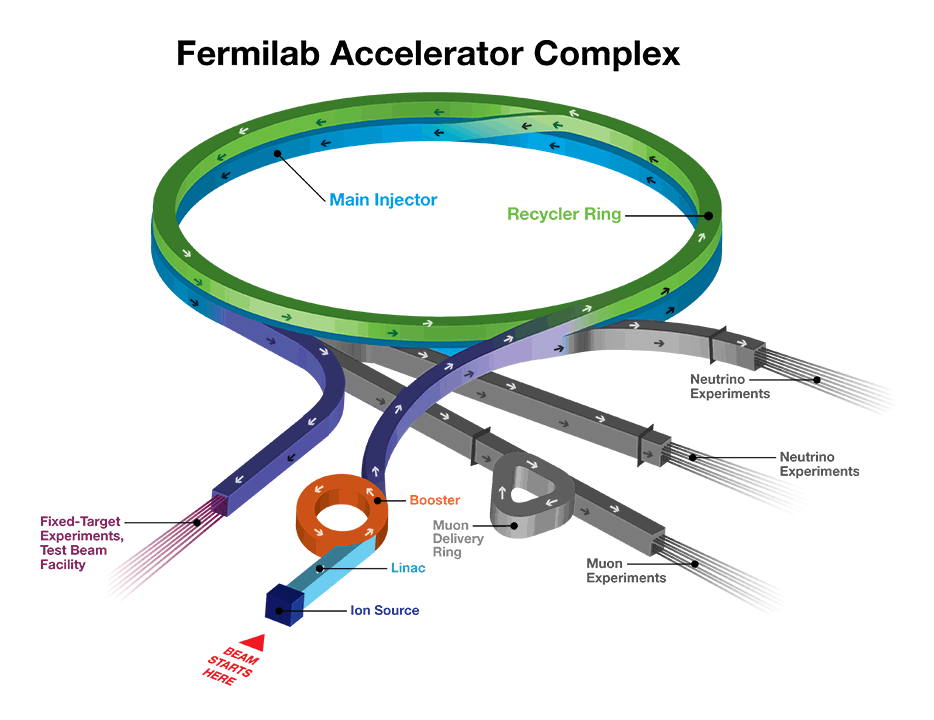
\includegraphics[width=\textwidth,height=\textheight,keepaspectratio]{Chapter-2/Images/AcceleratorFNAL.png}
\label{fig:Accelerator}
\caption{Layout of Fermilab Acellerator complex.}
\end{figure}

%\begin{comment}     
\begin{figure}
  \centering  	
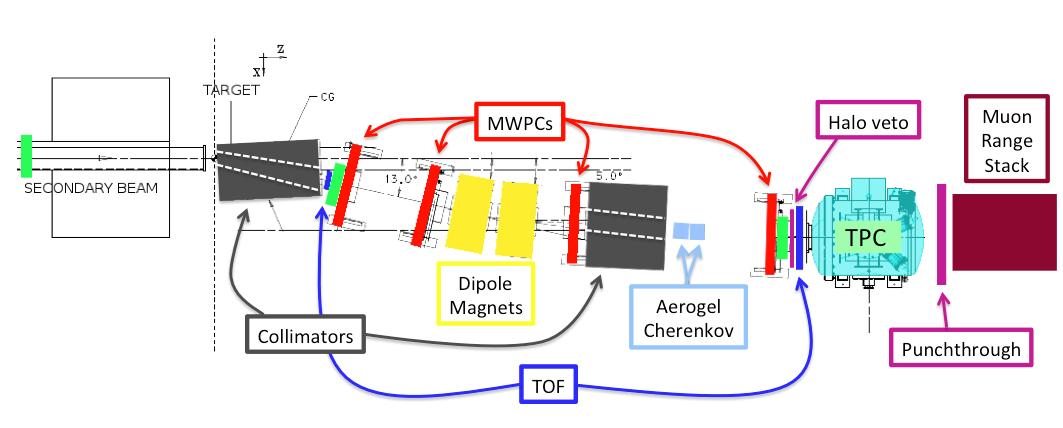
\includegraphics[width=\textwidth,height=\textheight,keepaspectratio]{Chapter-2/Images/Tertiary.png}
\label{fig:tert-layout}
\caption{Birds eye view of the LArIAT tertiary beamline. In grey: upstream and downstream collimators; in yellow: bending magnets in yellow; in red: wire chambers; in blue: time of flight; in green: liquid argon TPC volume; in maroon: muon range statck.}
\end{figure}


%%%%%%%%%%%%%%%%%%%%%%%%%%%%%%%%%%%%%%%%%%%%%%%%%%%%%%%%%%%%
\section{LArIAT Tertiary Beam Instrumentation}\label{sec:Instrumentation}

%%%%%%%%%%%%%%%%%%%%%%%%%%%%%%%%%%%%%%%%%%%%%%%%%%%%%%%%%%%%
The instrumentation of  LArIAT tertiary beam and the TPC components have changed several times during the three years of LArIAT data taking. The following paragraphs describe the components operational during the data taking period relevant to the hadron cross section measurements (a.k.a. Run II).

The components of the tertiary beamline instrumentation key for the hadron cross section analyses are the target and collimators system, the two bending magnets (in a similar configuration used for the  MINERvA T-977 test beam calibration~\cite{MinervaTestbeam}) a set of four wire chambers (WCs) and two time-of-flight scintillating paddles (TOF) and, of course, the LArTPC.  The magnets determine the polarity of the particles in the tertiary beam; the combination of magnets and wire chambers determine the particles momentum, which is used to determine the particle species in conjunction with the TOF.
A muon range stack downstream from the TPC and two sets of cosmic paddles configured as a telescope surrounding the TPC are also used for calibration purposes.


\subsection{Bending Magnets}\label{sec:Magnets}
%%%%%%%%%%%%%%%%%%%%%%%%%%%%%%%%%%%%%%%%%%%%%%%%%%%%%%%%%%%%
LArIAT uses a pair of identical Fermilab type ``NDB" electromagnets, recycled from the Tevatron's anti-proton ring \textcolor{red}{CITE CDF?}. 
The magnets are a fundamental piece of the LArIAT beamline as they are used in all the three tasks of the LArIAT beamline: the sign of the current in the magnet provide the selection of either positively or negatively charged particles, the value of the magnetic field is used in the momentum determination and the subsequent particle identification. 

We describe here the characteristics and response of one magnet. We expect the second one have a similar response, being identical in shape and with a similar history. The magnet aperture measures the gap dimensions to be 14.224~cm of height, 31.75~cm width, and  46.67~cm length.  The wire chambers aperture ($\sim$12.5~cm) is smaller than the magnet aperture, thus, only the central part of the magnet gap is utilized. The field is extremely uniform over this limited aperture and was measured with two Hall probes, both calibrated with nuclear magnetic resonance probes. The probes measured the excitation curve shown in Figure~\ref{fig:magnet_excitation}. 

\begin{figure}[!h]
\begin{centering}
\vspace{-0.3cm}
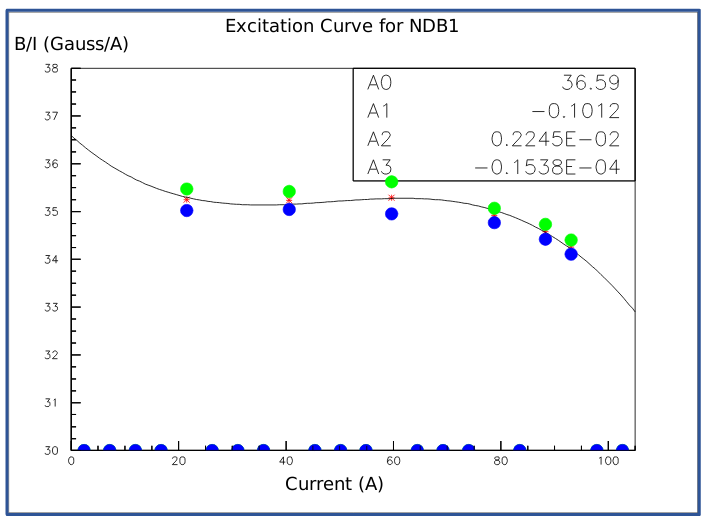
\includegraphics[height=3.0in]{Chapter-2/Images/ExcitationCurves.png}
\caption{
{ Magnetic field over current as a function of the current, for one NDB magnet (excitation curve). The data was collected using two Hall probes (blue and green). We fit the readings with a cubic function (black) to average of measurements (red) given in the legend.}
}
\label{fig:magnet_excitation}
\end{centering}
\end{figure}

The current being passed through the magnets at a given time is identical in both magnets. For Run II period, the current settings explored were 60A (B $\sim$0.21 T) and 100A (B $\sim$0.35 T) in both polarities. 
Albeit advantageous to enrich the tertiary beam composition with high mass particles such as kaons, we never pushed the magnets current over 100 A, not to incur in overheating.  During operation, we operated a air and water cooling system on the magnets and we remotely monitored the magnets temperature.
 
\subsection{Multi-Wire Proportional Chambers}\label{sec:MWPC}
%%%%%%%%%%%%%%%%%%%%%%%%%%%%%%%%%%%%%%%%%%%%%%%%%%%%%%%%%%%%
\begin{figure}[!h]
\begin{centering}
\vspace{-0.3cm}
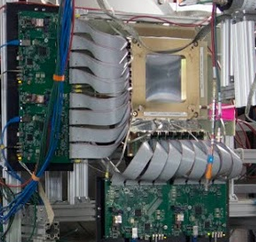
\includegraphics[height=2.3in]{Chapter-2/Images/WireChamber.png}
\caption{
{One of the four Multi Wire Proportional Chambers (WC) used in the LArIAT tertiary beamline.}
}
\label{fig:wirechamber}
\end{centering}
\end{figure}

LArIAT uses four Multi-Wire proportional chambers, or wire chambers (WC) for short, two upstream and two downstream from the bending magnets. The geometry of one chamber is shown in Figure~\ref{fig:wirechamber}: the WC effective aperture is a square of  12.8~cm perpendicular to the beam direction.  Inside the chamber, the 128 horizontal and 128 vertical wires hang at a distance of 1~mm from each other in a mixture of 85\% Argon and 15\% isobutane gas.  The WC operating voltage is between 2400 V and 2500 V. LArIAT wire chambers are an upgraded version of the Fenker Chambers~\cite{Fenker}, where an extra grounding improves the signal to noise ratio of the electronic readout.  

Two ASDQ chips~\cite{ASDQchip} mounted on a mother board plugged into the chamber serve as front end amplifier/discriminator. The chips are connected to a multi-hit TDC~\cite{Sten} which provides a fast OR output used as first level trigger. The TDC time resolution is 1.18~ns/bin and can accept 2 edges per 9~ns.  
The maximum event rate acceptable by the chamber system is of 1 MHz: this rate is not a limiting factor considering that the rate of the tertiary particle beam at the first wire chamber is estimated to be less than 15 kHz. A full spill of data occurring once per supercycle is stored on the TDC board memory at once and read out by a controller specially designed controller.  We use LVDS cables to carry both power and data between the controller and the TDCs and from the controller to the rest of the DAQ.  
%It is possible to program the time window for acceptance for hits, time offsets, front end threshold, and pulse shaping parameters through the controller via a USB from a PC or through an Ethernet connection.

\subsubsection{Multi-Wire Proportional Chambers functionality}\label{sec:MWPCfunc}


\subsection{Time-of-Flight System}\label{sec:TOF}
%%%%%%%%%%%%%%%%%%%%%%%%%%%%%%%%%%%%%%%%%%%%%%%%%%%%%%%%%%%%
Two scintillator paddles, one upstream to the first set of WCs and one downstream to the second set of WCs  form LArIAT  time-of-flight (TOF) detector system. 

 \textcolor{red}{find exact dimentsions}
The upstream paddle is made of a 10 x 6 x \textcolor{red}{?}~cm scintillator piece, read out by two \textcolor{red}{Hamamatsu 2 inch} PMTs mounted on the beam left side which collect the light from light guides mounted on all four edges of the scintillator. The downstream paddle dimensions are  14 x 14 x \textcolor{red}{?}~cm and it is read out by two \textcolor{red}{Hamamatsu 2 inch} PMTs on the opposite ends of the scintillator.
The relatively thin width on the beamline direction minimizes energy loss of the particles coming from the target in the scintillator material.

%\begin{figure}[!h]
%\begin{centering}
%\vspace{-0.3cm}
%\includegraphics[height=2.3in]{Chapter-2/Images/tofdelay.png}
%\caption{
%{\scriptsize \sf Pictures of the TOF system as was deployed during Run-I and Run-II data taking. The left image is of the upstream TOF paddle and the right image is of the downstream TOF paddle }
%}
%\label{fig:TOFSystemRunIandII}
%\end{centering}
%\end{figure}



The CAEN 1751 digitizer is used to digitize the TOF PMTs signals at a sampling rate of 1 GHz. The 12 bit samples are stored in a circular memory buffer. At trigger time, data from the TOF PMTs are recorded to output in a 28.7 $\mu$ second windows starting  approximately 8.4 $\mu$sec before the trigger time. 



\subsubsection{TOF functionality}\label{sec:MWPCfunc}


The TOF signals rise time (10-90\%) is 4 ns and a full width, half-maximum of 9 ns consistent in time. The signal amplitudes from the upstream TOF and  downstream TOF are slightly different:  200 mV for the upstream PMTs but only 50 mV for downstream PMTs. The time of the pulses was calculated utilizing an oversampled template derived from the data itself. We take the pulse pedestal from samples far from the pulse and subtract it to the pulse amplitude. We then stretch vertically a template to match the pedestal-subtracted pulse amplitude and we move it horizontally to find the time. With this technique, we find a pulse time-pickoff resolution better than 100 ps.  The pulse pile up is not a significant problem given the TOF timing resolution and the rate of the particle beam.  Leveraging on the pulses width uniformity of any given PMT (sigma of 400 ps),  we flag events where two pulses overlap as closely in time as 4 ns with an 90\% efficiency according to simulation. 


We combine the pulses from the two PMTs on each paddle to determine the particles' arrival time by averaging the time measured from the single PMT, so to minimize errors due to optical path differences in the scintillator.  However, a time spread of approximately 300~ps is present in both the upstream and downstream detectors, likely due to transit time jitter in the PMTs themselves.  There is no evidence of systematic timing drift over long data-taking periods such as 3-4 months: the maximum variation of the average time differences between pairs of PMTs reading out the same scintillator is of the order of 150~ps.

\textcolor{red}{calculated TOF with error}


%%%%%%%%%%%%%%%%%%%%%%%%%%%%%%%%%%%%%%%%%%%%%%%%%%%%%%%%%%%%
\subsection{Punch-Through and Muon Range Stack Instruments}\label{sec:MuRS}
%%%%%%%%%%%%%%%%%%%%%%%%%%%%%%%%%%%%%%%%%%%%%%%%%%%%%%%%%%%%

The punch-thorough and the muon range stack (MuRS) detectors are located downstream of the TPC. These detectors provide a sample of  TPC crossing tracks without relying on TPC information and can be used to improve particle ID for  muons and pions with momentum higher than  450 MeV/c.

The punch-thorough is simply a \textcolor{red}{? x ? x ?}~cm scintillator piece, read out by \textcolor{red}{ two? Hamamatsu? 2? inch} PMTs. 
The MuRS is a segmented block of steel with four slots instrumented with scintillation bars. The four steel layers in front of each instrumented slot are 2 cm, 2 cm, 14 cm and 16 cm wide in the beam direction. Each instrumented slot is equipped with four scintillation bars each, positioned vertically in the direction orthogonal to the beam. Each scintillator bar measures  \textcolor{red}{? x ? x 2}~cm and it is read out by  \textcolor{red}{ two? Hamamatsu? 2? inch} PMTs.  

The signals from both the punch-thorough and the MuRS PMTs are digitized in the CAEN V1740, same as the TPC; the details of this discriminator are laid out in~\ref{sec:TPCCharge}. It is worth noticing that the sampling time of the CAEN V1740 is slow (of the order of 128 ns), so pulse shape information from the PMT is lost.
Punch-thorough and MuRS hits are formed utilizing the OR between the PMTs digital discriminator signals under threshold at a given time, where we obtain the threshold for each PMT directly on data distributions.



%%%%%%%%%%%%%%%%%%%%%%%%%%%%%%%%%%%%%%%%%%%%%%%%%%%%%%%%%%%%
\subsection{LArIAT Cosmic Ray Paddle Detectors}\label{sec:CosmicRayPaddle}
%%%%%%%%%%%%%%%%%%%%%%%%%%%%%%%%%%%%%%%%%%%%%%%%%%%%%%%%%%%%
Besides on beam data, LArIAT also triggers on cosmic rays events by using two sets of cosmic ray paddle detectors (a.k.a. ``cosmic towers".) The cosmic towers frame the LArIAT cryostat, as one sits in the downstream left corner and the other sits in the upstream right corner of the cryostat. Two paddle sets of four scintillators pieces each, an upper and a lower set, make up each cosmic tower. 
Of the four paddles, a couple of two matched paddles stands upright while the a second matched pair lies across the top of the assembly in the top sets (or across the bottom of the assembly in the bottom sets). The horizontal couple is used as a veto for particles traveling from the TPC out.  The four signals  from the vertical paddles along one of the body diagonals of the TPC are combined in a logical ``AND''. This allows to select cosmic muons crossing the TPC along one of its diagonals.  Cosmic ray tracks crossing both anode and cathode populate the events triggered this way. This particularly useful sample of tracks (which we can safely assume to be associated with ~5 GeV muons MIPs) can be used for many tasks; for example, we use anode-cathode piercing tracks to cross check the TPC electric field on data (see \ref{ch:AppendixC}), to calibrate the charge response of the TPC wires for the full TPC volume and to measure the electron lifetime in the chamber \textcolor{red}{ ADD reference to different chapters}.

%%%%%%%%%%%%%%%%%%%%%%%%%%%%%%%%%%%%
All the paddles are $3.02~cm$ thick and are  trapezoidal in shape. The paddles come in two sizes: the smaller version has bases $32.2~cm$ and $26.7~cm$, and $61.0~cm$ height, while the bigger version has bases $33.2~cm$ and $27.0~cm$, and $70.8~cm$ height.  A Zener-diode Hamamatsu H5783 PMT collects the light from a wavelength-shifting optical fiber which runs along one of the long sides of each paddle.
A custom-made PMT Amplifier and Discrimination (PAD) circuit mounted at one end of the paddle collects signals from the PMTs and sends them to the Control and Concentrator Unit (CCU). We use the same connection to  power the PMT, control voltage and threshold, and output the PMT signal as logic ECL pulse.
We retrieved the scintillation paddles from the decommissioning of the CDF detector at Fermilab and we used only the paddles with a counting efficiency greater than 95\% and low noise at working voltage. The measured trigger rate of the whole system is $0.032Hz$, corresponding to $\sim 2$ muons per minute.


\begin{figure}[h!]
\centering
 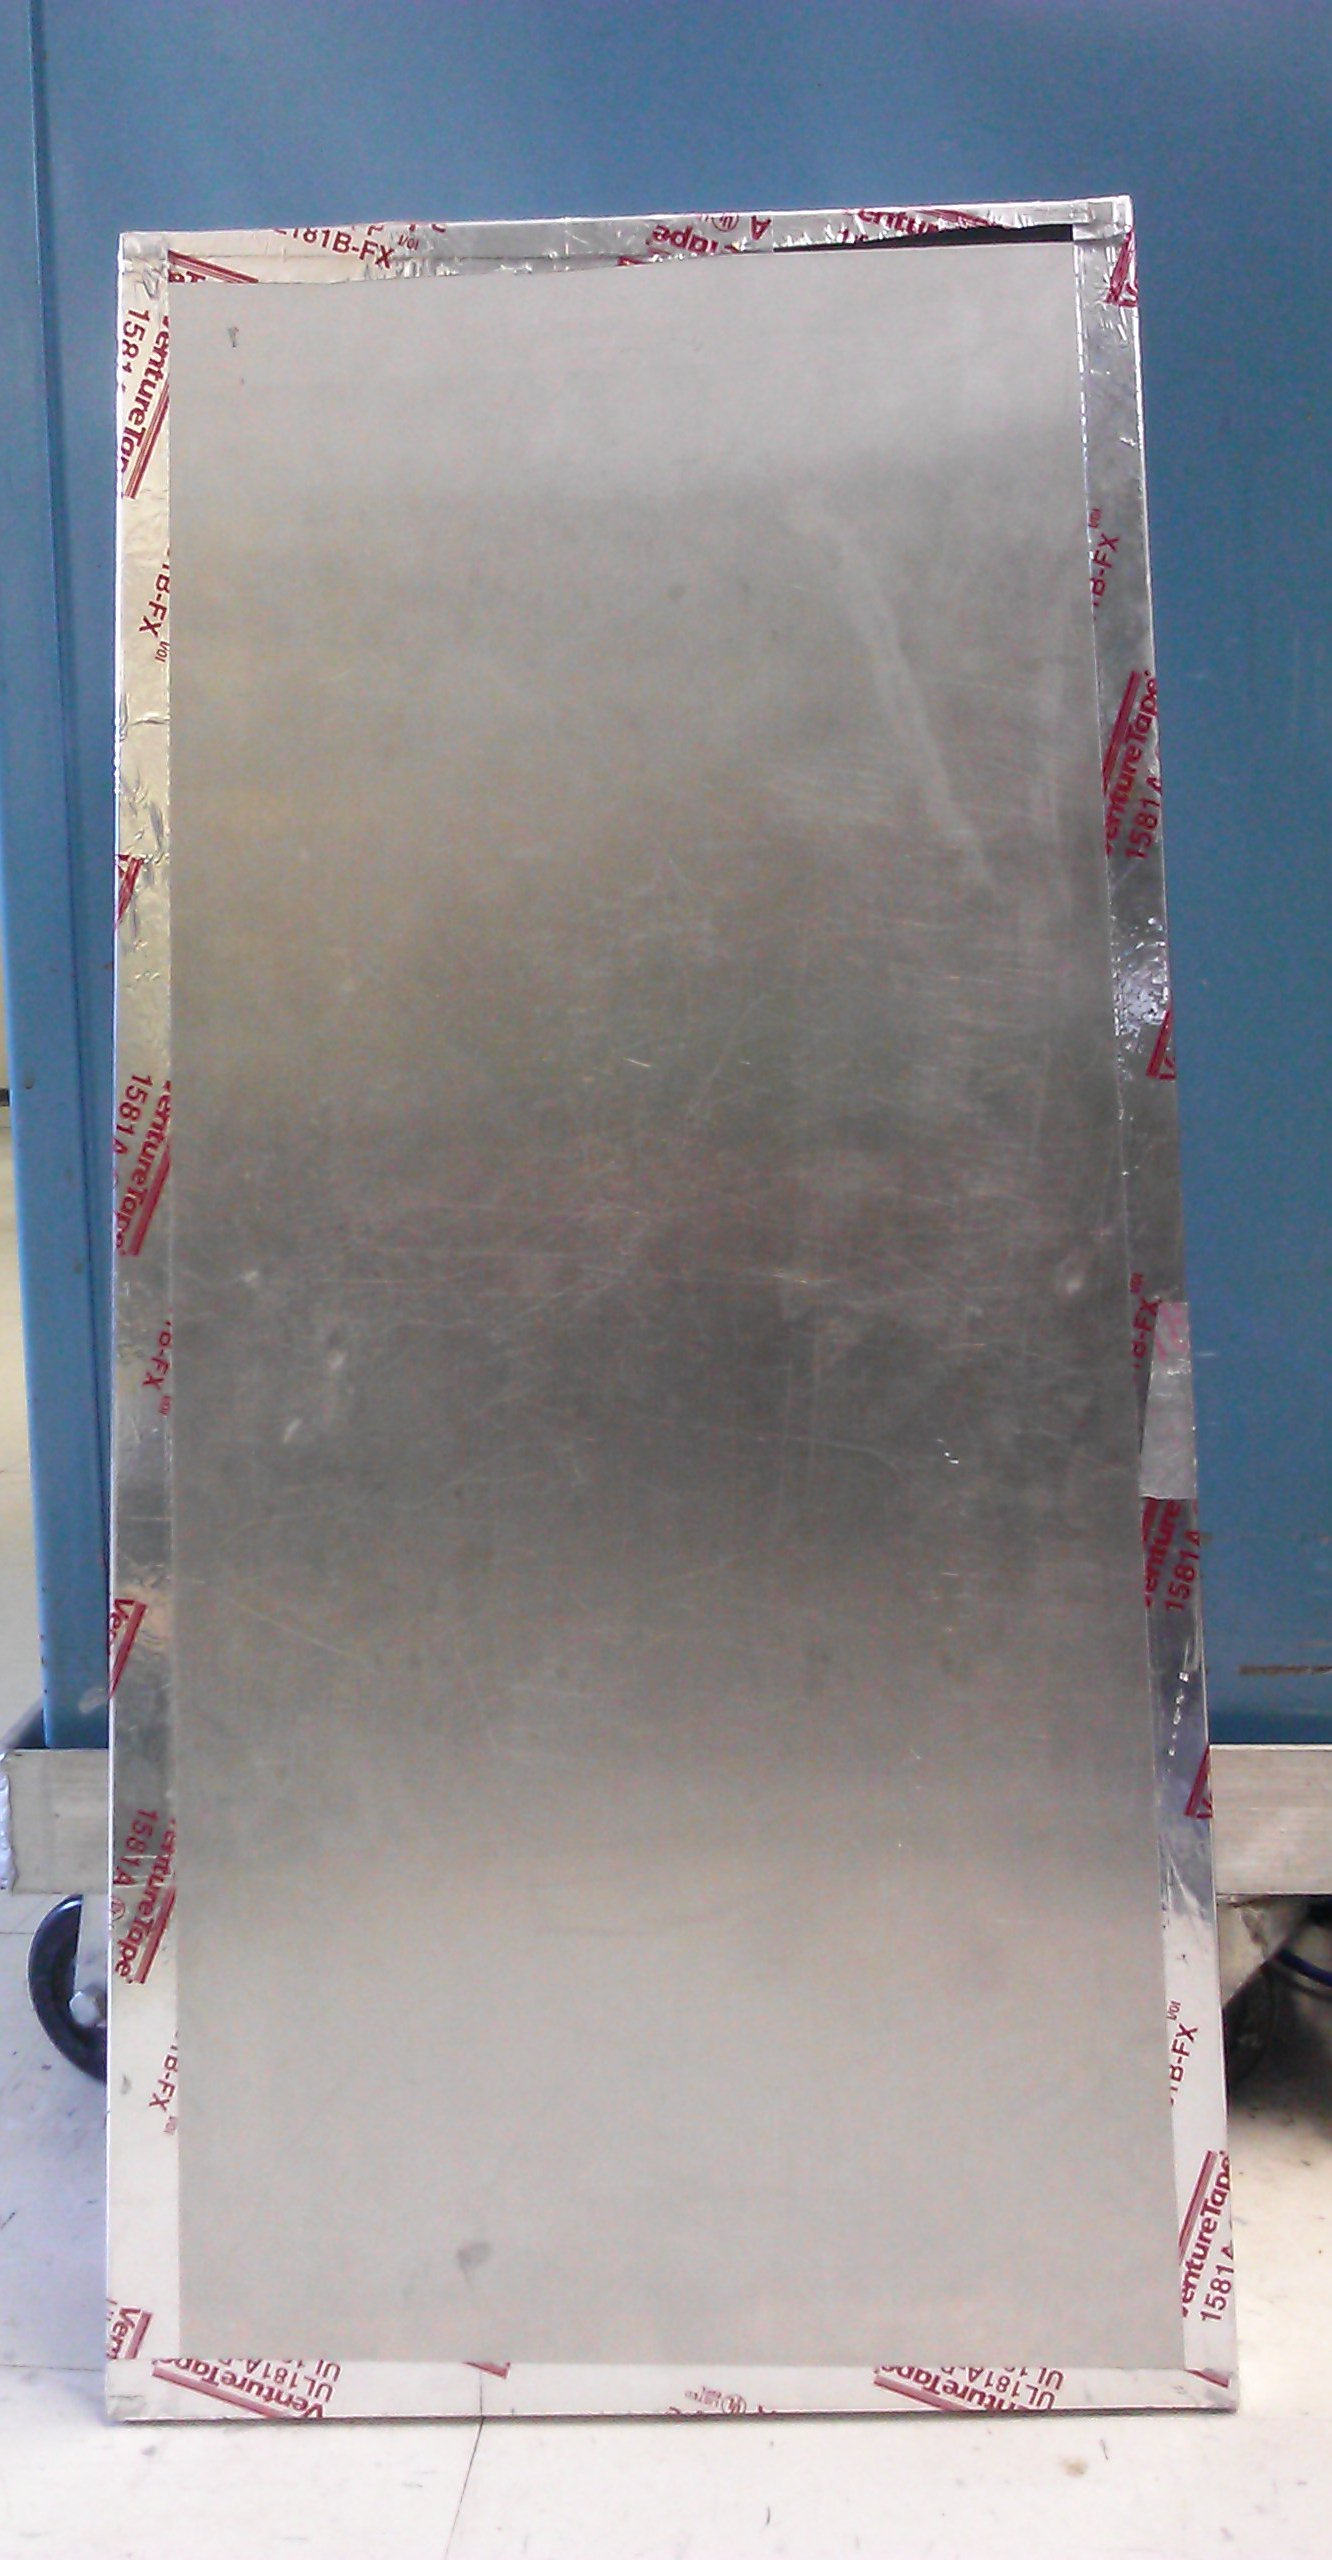
\includegraphics[angle=90,width=0.7\textwidth]{Chapter-2/Images/Cosmic_Paddle.jpg}
\caption{Photograph of one of the scintillation counters used in the cosmic towers. } 
\label{pic:cosmicpaddle}
\end{figure}






\section{In the Cryostat}
\subsection{TPC: Charge Collection}\label{sec:TPCCharge}
\subsection{TPC: Light Collection System}\label{sec:TPCLight}
The mechanism of particle detection in argon other than drift electrons is the collection of scintillation photons.  Over the course of LArIAT three years of data taking, the light collection system changed several times. We describe here the light collection system for Run II. Two PMTs, a 3-inch diameter Hamamatsu R-11065 and 2-inch diameter ETL D757KFL~\cite{lightsys-pmttests}, as well as three SiPMs arrays (two Hamamatsu S11828-3344M 4x4 arrays and one single-channel SensL MicroFB-60035 ) are mounted on the PEEK support structure. PEEK screws into an access flange as shown in Figure~\ref{lightsys_pmts}, on the anode side, leaving  approximately 5~cm of clearance from the collection plane.  

%------------------------------------------
\begin{figure}
\centering
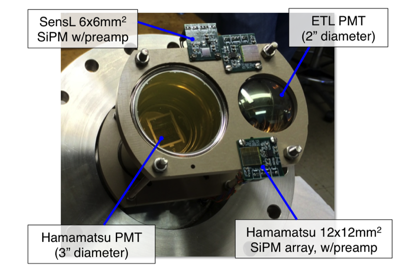
\includegraphics[height=2.2in]{Chapter-2/Images/lightsys_pmts.png}
\hspace{1cm}
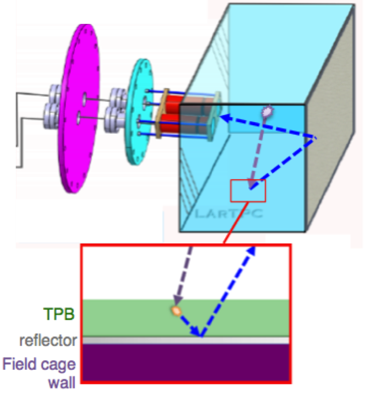
\includegraphics[height=2.2in]{Chapter-2/Images/lightsys_wls.png}
\caption{LArIAT's photodetector system for observing LAr scintillation light inside the TPC (left), and a simplified schematic of VUV light being wavelength-shifting along the TPB-coated reflecting foils (right).}
\label{lightsys_pmts}
\end{figure}
\begin{figure}
\centering
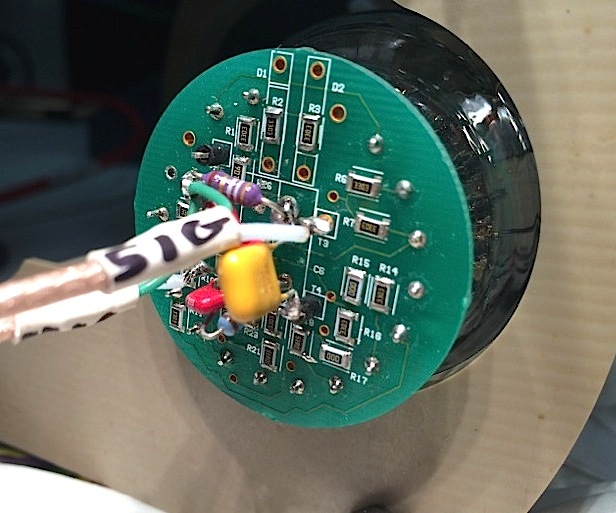
\includegraphics[height=0.25\textheight]{Chapter-2/Images/lightsys_etlbase.jpeg}
\hspace{0.5cm}
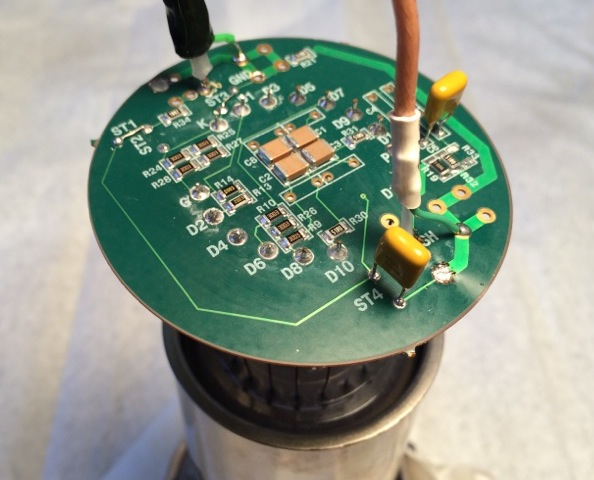
\includegraphics[height=0.25\textheight]{Chapter-2/Images/lightsys_hmmbase.jpg}
\caption{\label{voltagedividers}Photos of the voltage divider bases for the ETL PMT (left) and the Hamamatsu PMT (right) used in Run-II.  The cable connections to the bases seen here were used for powering and testing prior to installation.  The yellow through-hole signal coupling capacitors seen on both bases are 18~nF (X7R) and are rated to 2~kV.}
\end{figure}
%------------------------------------------
Liquid argon scintillates in vacuum-ultraviolet (VUV) range at 128 nm; since cryogenic PMTs are not sensitive to VUV wavelengths, we need to shift the light in a region visible to the PMTs. In LArIAT, the wavelength shifting is achieved by installing on the four walls of the TPC highly-reflective VIKUITY dielectric substrate foils coated with a thin layer of tetraphenyl-butadiene (TPB) (see Figure ~\ref{lightsys_foils}). One or more visible photons  are emitted and reflected into the chamber during the interaction of a VUV photon interacts with the TPB. Thus, the light yield is increased and made more uniform across the TPC active volume, allowing the possibility of light-based calorimetry (under study).

%------------------------------------------
%\begin{figure}
%\centering
%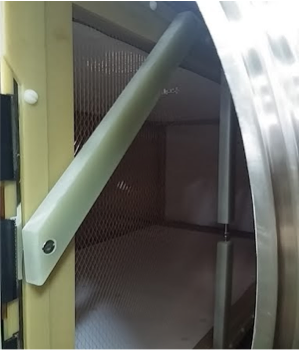
\includegraphics[scale=1.3]{Chapter-2/Images/lightsys_foils.png}
%\caption{\label{lightsys_foils}The TPB-coated reflector foils mounted to the TPC field cage walls as viewed through the front cryostat opening. {\textcolor{red}{Better pictures needed.}}}
%\end{figure}
%------------------------------------------

For Run II, we coated both  the windows of the ETL PMT and SensL SiPM  with a thin layer of TPB. In doing so, some of the VUV scintillation light converts into visible right at the sensor faces, keeping information on the direction of the light source. Information about the light directionality is lost for light reflected on foils, as the reflection is uniform in angle. For Run-II, the voltage dividers for the PMTs were configured for positive bias with a DC-coupled anode (AC-coupled anode with grounded photocathode) to minimize induced noise on the TPC wires and modify the PMT bases accordingly.  


\subsection{Cryogenics and Purity Control}\label{ch:Cryo}
LArIAT repurposed the ArgoNeuT cryostat \cite{argoneut} in order to use it in a beam of charge particles. We also added a new process piping and a new liquid argon filtration system in FTBF.
Inside the LArIAT experimental hall, the cryostat sits on the beam of charge particles with its horizontal main axis oriented parallel to the beam.

Two volumes make up LArIAT cryostat, shown in Figure \ref{fig:LArIATCryoStat}: purified liquid argon fills the inner vessel, while the outer volume insulates it with a vacuum jacket equipped with layers of aluminized mylar superinsulation. The inner vessel is a cylinder of 130~cm length and 6.2~cm diameter, containing about 550~L of LAr, corresponding to a mass of 0.76 ton. We run the signal cables for the LArTPC and the high voltage feedthrough through a ``chimney'' at the top and mid-length of the cryostat.


\begin{figure}[htb]
\centering
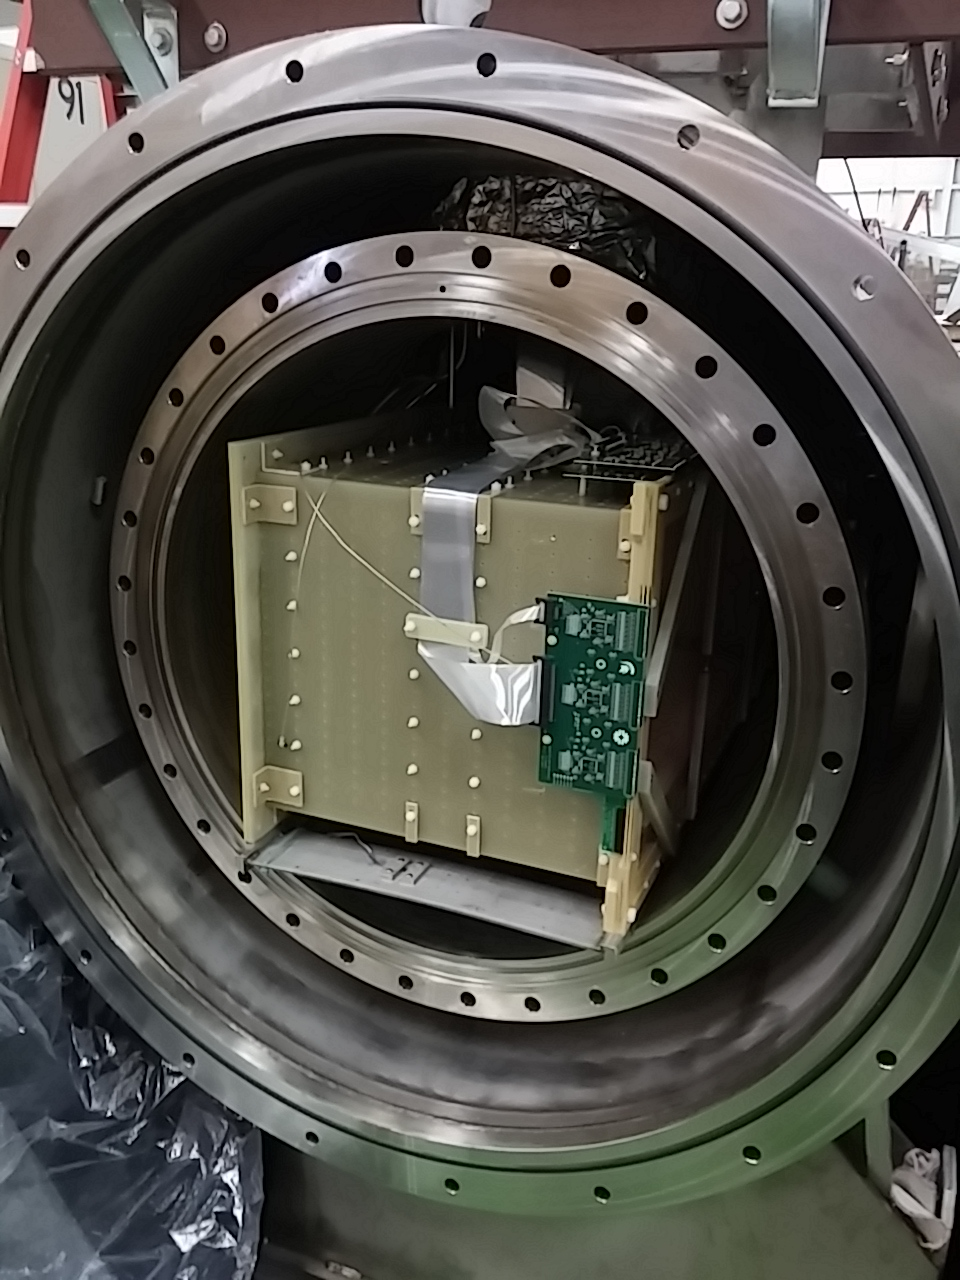
\includegraphics[scale=0.18]{Chapter-2/Images/Cryostat1.jpg}
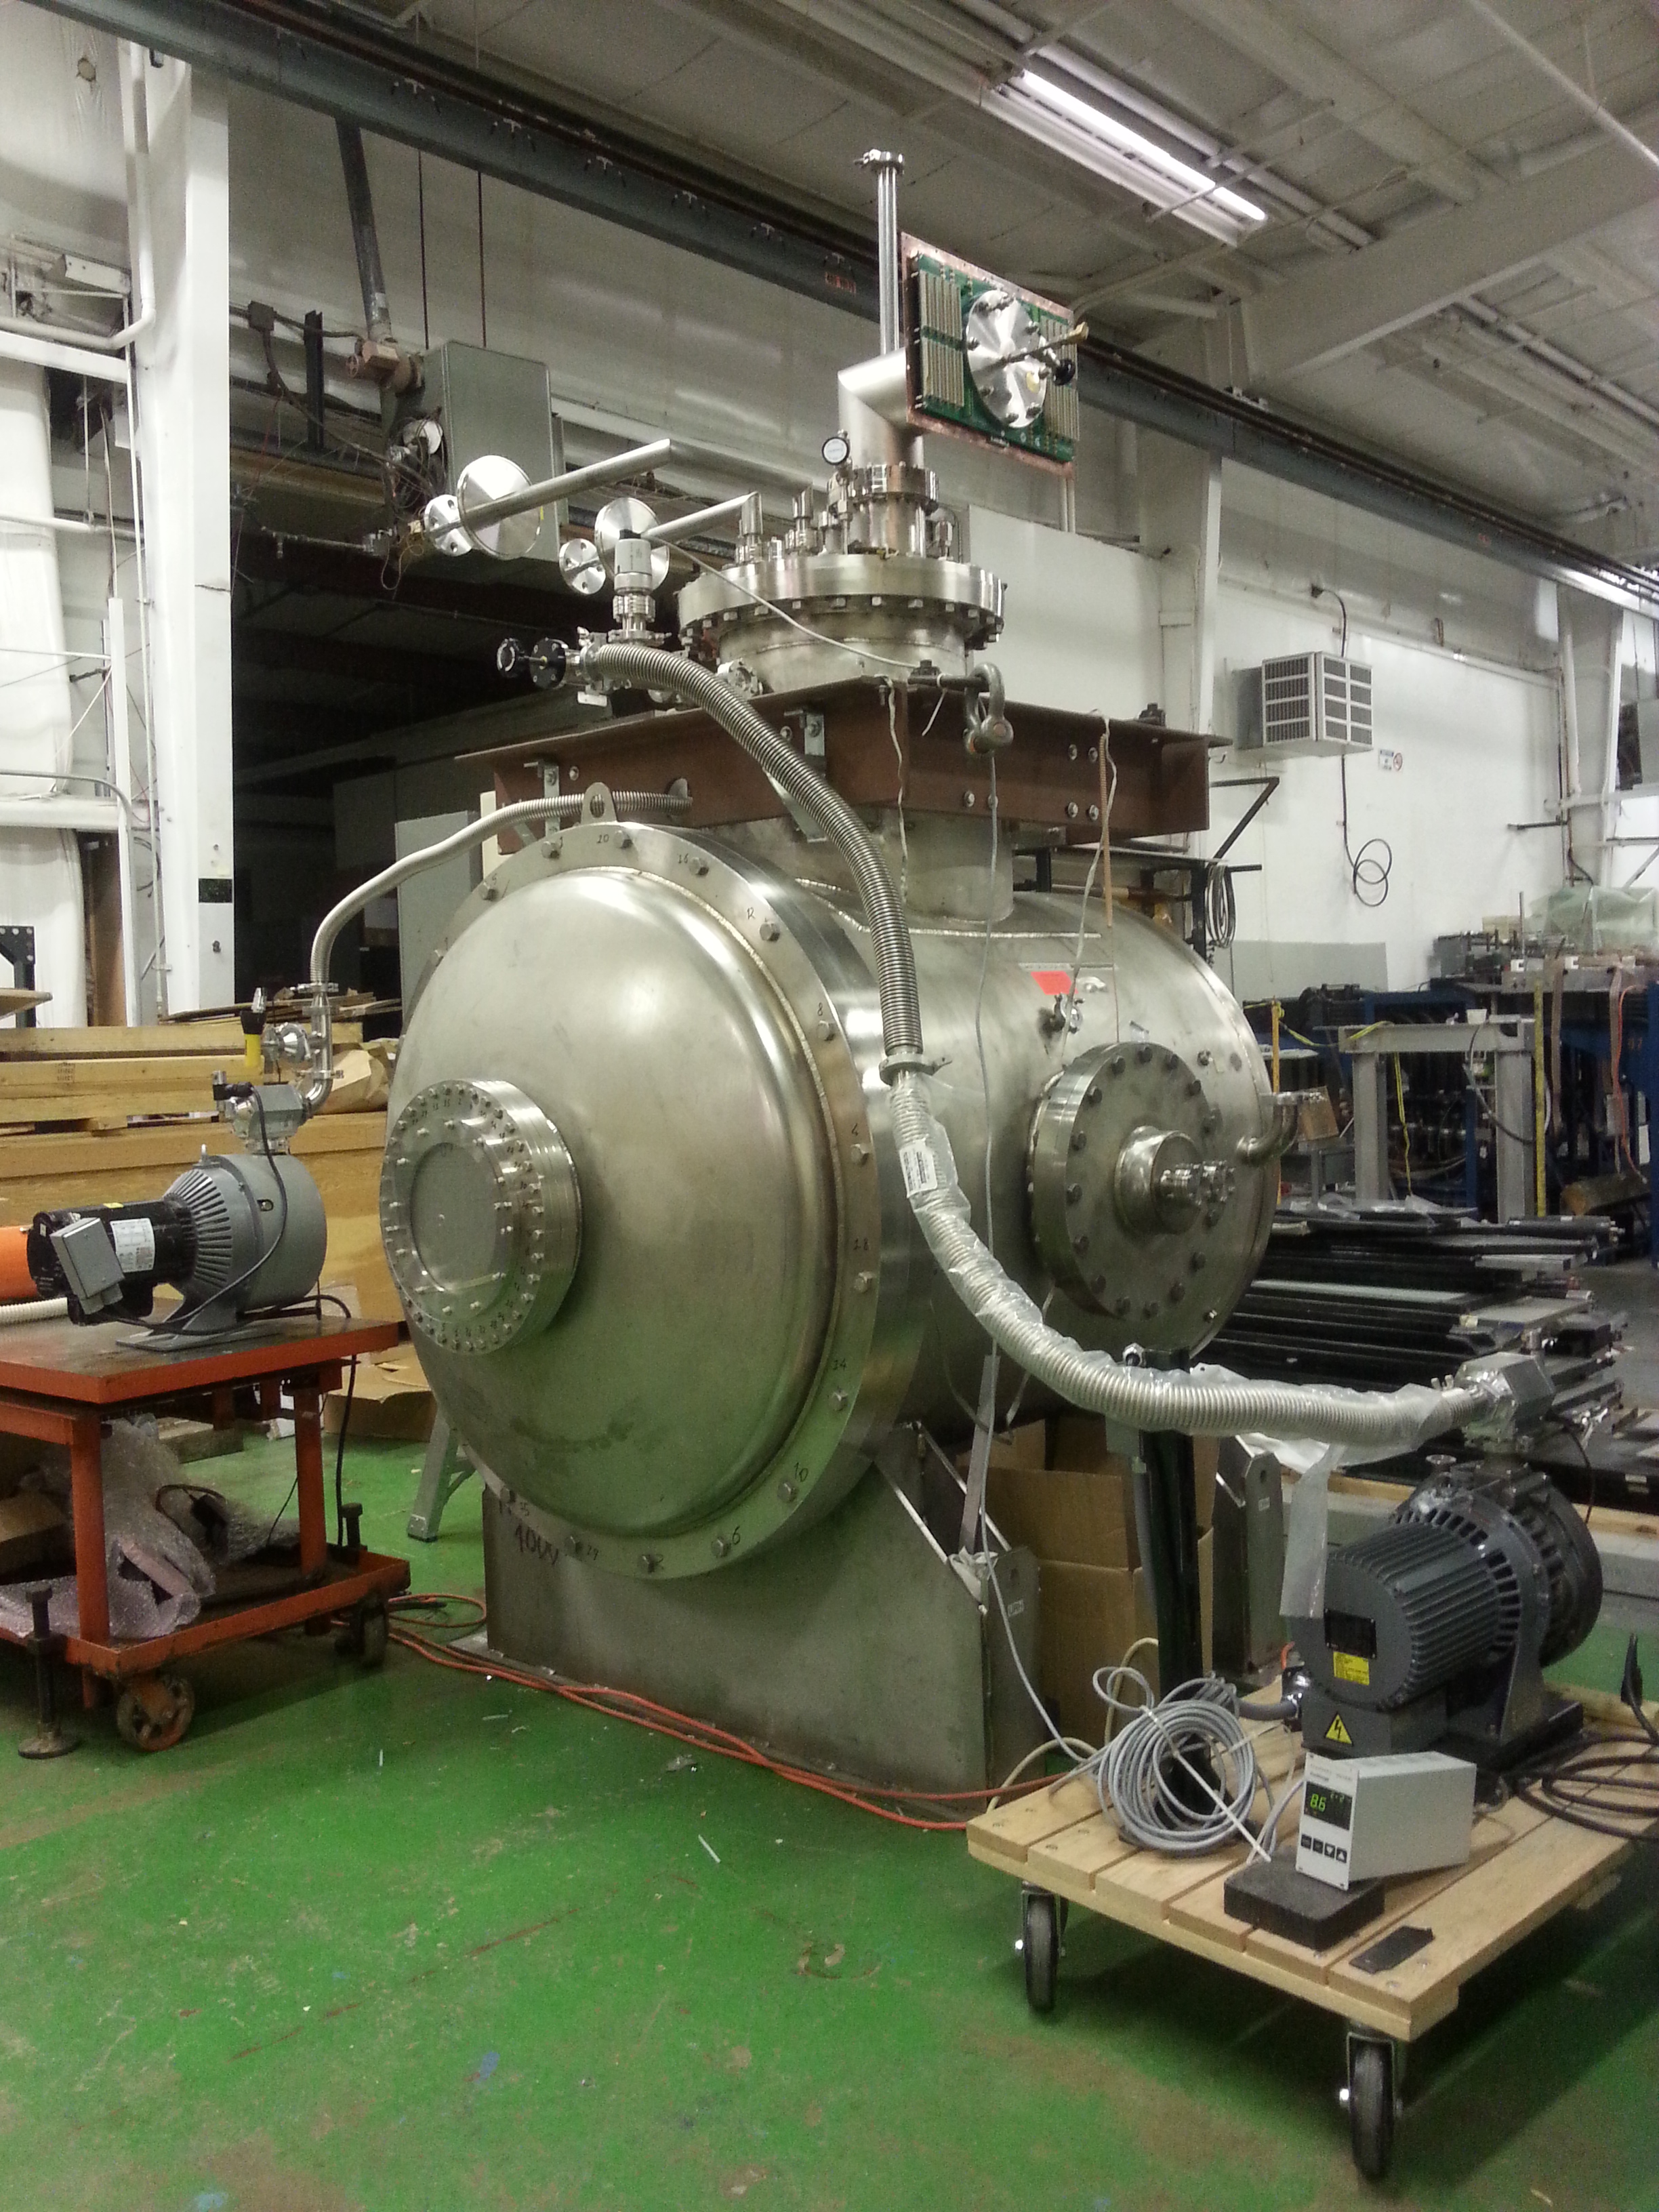
\includegraphics[scale=0.07]{Chapter-2/Images/Cryostat2.jpg}
\caption{\emph{(left)} The LArIAT cryostat open with the TPC placed in the inner volume. \emph{(right)} The LArIAT cryostat fully sealed during initial commissioning prior to installation at Fermilab Testbeam Facility.Access to the internal volume is possible by opening the upstream end caps of the inner and outer vessels. }
\label{fig:LArIATCryoStat}
\end{figure}

Given the different scopes of the ArgoNeuT and LArIAT detectors, we made several modification to the ArgoNeuT cryostat in order to use it in LArIAT. In particular, the modification  shown in Figure \ref{fig:LArIATCryoMods} were necessary to account for the beam of charged particles entering the TPC and to employ the new FTBT liquid argon purification system. 
We added a ``beam window'' on the front outer end cap and an ``excluder'' on the inner endcap, with the scope of minimizing the amount of dead material upstream of the TPC's active volume.  Doing so, we reduced the amount of uninstrumented material before the TPC from $\sim$ 1.6 radiation lengths ($X_{0}$) (ArgoNeuT) to less than 0.3 $X_{0}$ (LArIAT). To allow studies of the scintillation light, we added a side port feedthrough which enables the mounting of the light collection system, as well as the connections for the corresponding signal and high-voltage cables (see Section \ref{sec:TPCLight}).  We modified the bottom of the cryostat adding Conflat and ISO flange sealing to connect the liquid argon transfer line to the new argon cooling and purification system.



\begin{figure}[htb]
\centering
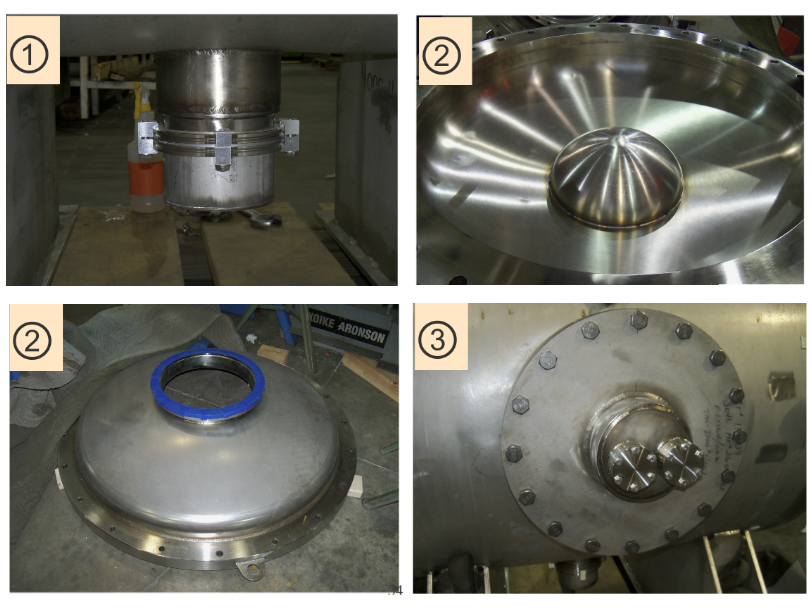
\includegraphics[scale=0.35]{Chapter-2/Images/CryoMods.png}
\caption{Pictures of the modified components of the cryostat. $1)$ The addition of an outlet to the bottom of the cryostat to allow connections to the purification system; $2)$ The ``beam-window'' on the outer endcap and the concave inner surface of the inner endcap (referred to as the excluder) to reduce the amount of material through which beam particles must travel before entering the TPC; $3)$ The modified side port for the LArIAT light collection system.}
\label{fig:LArIATCryoMods}
\end{figure}

%%%%%%%%%%%%%%%%%%%%%
As in any other LArTPC, argon purity is a crucial parameter for LArIAT. Indeed, the presence of contaminants effects both the basic working principles of a LArTPC: electronegative contaminants such as oxygen and water decrease the number of ionization electrons collected on the wires after drifting through the volume, while contaminants such as Nitrogen decrease the light yield from scintillation light, especially in its slow component.

The argon path

LArIAT argon is less than  1~ppm of oxygen, water and nitrogen contaminants.
monitor with the use of  commercial gas analyzer.
LArIAT makes use of LAr supplies from a vendor 

LArIAT is supplied with liquid argon from a commercial dewar positioned outside of the experimental enclosure.  
Liquid argon is delivered by a vendor with a specified maximum contamination of 2 parts per million (ppm) oxygen, 3.5~ppm water, and 10~ppm nitrogen which we 


In practice, the delivered argon has much less than 1~ppm of all these contaminants.  Even such apparently low levels of contamination are too large to effectively drift ionization electrons, so filtration of the argon is required to achieve oxygen and water contamination at the level of 100 parts per trillion (ppt) or better. 

The argon is delivered from the commercial dewar to the cryostat through 2.54~cm diameter schedule 10 stainless steel piping.  The piping was insulated with 20.32~cm of polyurethane foam by the manufacturer.  The piping was cleaned to remove oil and grease before being welded into the system. The argon then passes through LArIAT's argon filtration system which is based on the Liquid Argon Purity Demonstrator (LAPD)~\cite{LAPD} design. The purification system consists of a single 77~liter filter which is filled halfway with a 4A molecular sieve supplied by Sigma-Aldrich~\cite{sigma-aldrich} that primarily removes water contamination but can also remove small amounts of nitrogen and oxygen. The remaining volume of the filter contains BASF~CU-0226~S, a highly dispersed copper oxide impregnated on a high surface area alumina, to remove oxygen~\cite{basf} and to a lesser extent, water.  The filter is insulated with a vacuum jacket and aluminum radiation shields.  The filter media are regenerated in place using heated gas, as was done for LAPD. The filter media are very efficient at removing oxygen and water and the argon is pure enough after a single pass through the media to allow several millisecond electron drift lifetimes in the TPC. 

From the filter the argon is directed into the inner cryostat via a liquid feedthrough on the top of the cryostat. The argon level, temperatures, and pressures are continuously monitored during operation both in the commercial dewar supplying the argon as well as the levels inside the cryostat, as shown on the top of Figure \ref{fig:LArIATCryoMonitor}. The argon in the cryostat is allowed to boil and vent to the atmosphere during operation and the argon level is monitored via the level probes. Flow of argon into the cryostat is enabled whenever the liquid level goes below a predetermined value to ensure that the TPC high voltage feedthrough and cold electronics are always submerged. During normal operations, the liquid level inside the cryostat is replenished several times per day, as can be seen by the cycle of the liquid level and valve positions shown at the bottom of Figure \ref{fig:LArIATCryoMonitor} 

\begin{figure}[htb]
\centering
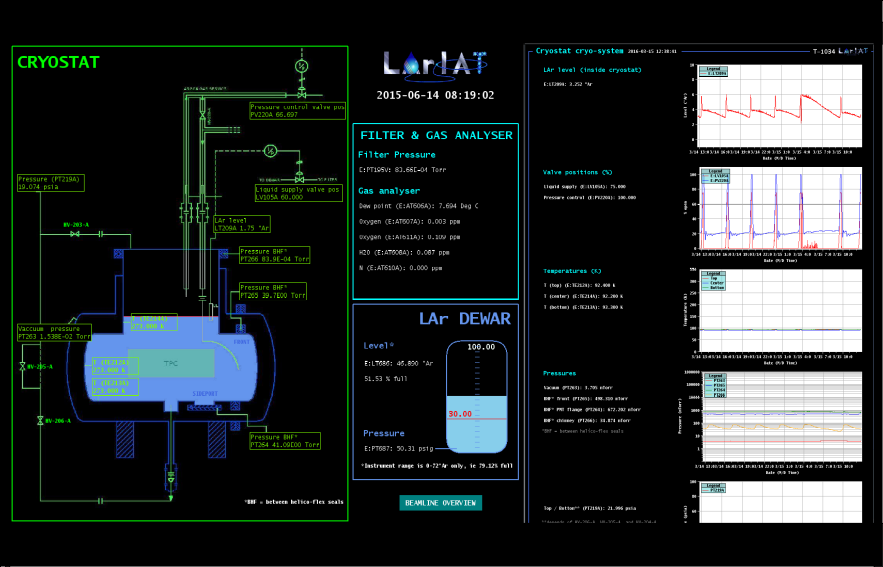
\includegraphics[scale=0.35]{Chapter-2/Images/CryoMonitor.png}
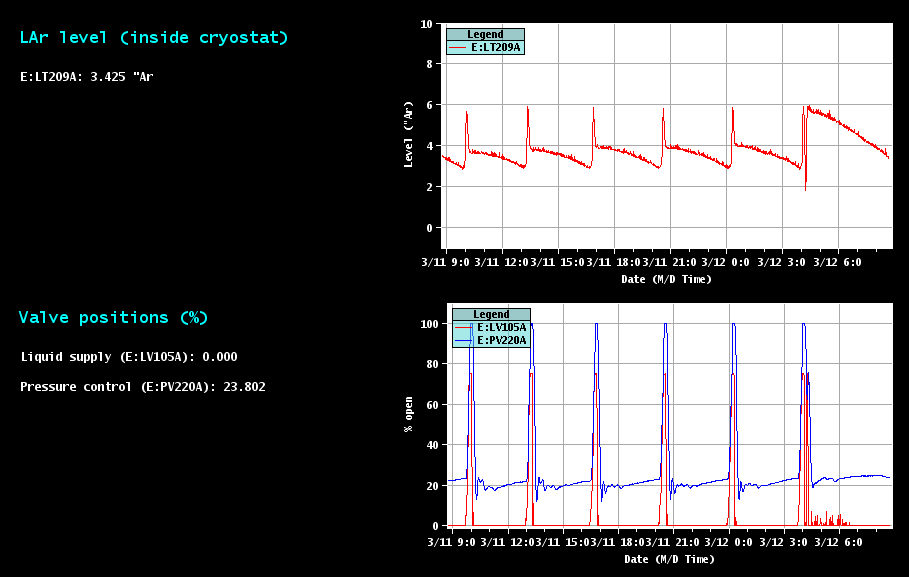
\includegraphics[scale=0.34]{.Chapter-2/Images/CryoMonitor2.png}
\caption{\emph{(top)} Screenshot of the LArIAT cyrosystem monitoring page showing the levels of the argon both inside the cryostat and in the supply dewar as well as the monitored levels plotted over a twenty-four hour period. \emph{(bottom)} Plots showing the liquid argon level inside the cryostat as well as the corresponding liquid valve which allows argon to flow into the cryostat and the level drops due to boiling. The frequency of the typical fill/vent cycle can be seen with the typical time between fills being slightly more than 3 hours.}
\label{fig:LArIATCryoMonitor}
\end{figure}



\section{Trigger and DAQ}
\section{Control Systems}
